\chapter{数値実験}
\label{chap:experiment}

本章では,提案したアルゴリズムの有効性を検証するための実験を行う.
\ref{sect:exp-artificial}では,有効性の検証とともに,
\ref{subsect:computational-complexity-of-incremental-algorithm}と
\ref{subsect:computational-complexity-of-decremental-algorithm}で
行った理論的な解析結果との関連を示す.
\ref{sect:exp-realnet}では,提案したアルゴリズムの応用を想定した実験を行う.

\section{人工ネットワークに対する結果}
\label{sect:exp-artificial}

本説では,以下の項目について実験を行い,その結果について考察する.
\begin{enumerate}
\item Brandesのアルゴリズムとの比較
\item 距離および経路数を更新した頂点ペアの数および
  ペア依存度を更新した頂点ペアの数と実行時間の関係
\item 媒介中心性が実際に変化した頂点の数と更新した頂点の数
\end{enumerate}

この実験では,次の三種類の人工ネットワークを対象とする.
\begin{enumerate}
\item ランダム正則グラフ
\item Erd\H{o}s--R\'{e}nyiモデル\cite{Erdos1959}
\item Barab\'{a}si--Albertモデル\cite{Barabasi1999}
\end{enumerate}

\subsection{頂点数の増加と実行時間の変化}

\begin{enumerate}
\item 再計算:辺が挿入または削除される度にBrandesのアルゴリズム(アルゴリズム\ref{algo:brandes})で媒介中心性を再計算する
\item 更新:辺が挿入された場合アルゴリズム\ref{algo:incremental-algorithm}で媒介中心性を更新し,削除された場合アルゴリズム\ref{algo:decremental-algorithm}で媒介中心性を更新する
\end{enumerate}

図\ref{fig:exp-artificial-order}は各アルゴリズムの実行時間を比較したものである.
各ネットワークの平均次数はおよそ$4$である.それぞれの頂点数について,
100個のネットワークに対する実行時間の最大値および平均値を計算している.
図\ref{fig:exp-artificial-order}より,三種類のネットワーク全てに対して,
頂点数が増加するとともに更新の平均実行時間が再計算のものと比べて短くなっていることが分かる.
頂点数の増加とともに,ペア依存度を再計算する必要がある頂点が比較的少なくなることが理由と考えられる.

\begin{figure}[tb]
  \centering
  \includegraphics[width=\linewidth]{exp-artificial-order.pdf}
  \caption{頂点数に対する実行時間の比較}
  \label{fig:exp-artificial-order}
\end{figure}

\subsection{更新の量と実行時間の関係}

提案したアルゴリズムのような,オンラインアルゴリズムの性能を評価するためには,
アルゴリズムによって更新した要素の数を考慮する必要がある.
\cite{Ramalingam1996,Lee2012,Pontecorvi2014}
ここでは,更新した頂点ペア数と実行時間の関係を実験によって明らかにする.
さらに,
\ref{subsect:computational-complexity-of-incremental-algorithm}と
\ref{subsect:computational-complexity-of-decremental-algorithm}で
行った理論的な解析結果と,実験データの挙動が一致するか検証する.

図\ref{fig:exp-artificial-update}は最短経路およびペア依存度を更新した頂点ペア数と実行時間の関係を表す.
頂点数を$1000$,平均次数は$4$または$64$とし,$100$回の更新を行った.
図\ref{fig:exp-artificial-update}より,更新した頂点ペア数が少ないと,実行時間が短くなることが分かる.
さらに,次数が大きいと実行時間が長くなる.この性質は理論的な解析結果と矛盾しない.

\begin{figure}[tb]
  \centering
  \includegraphics[width=\linewidth]{exp-artificial-update.pdf}
  \caption{更新した頂点ペアの数に対する実行時間}
  \label{fig:exp-artificial-update}
\end{figure}

\subsection{媒介中心性を更新した頂点の数と変化した頂点の数の関係}

\ref{subsect:computational-complexity-of-incremental-algorithm}と
\ref{subsect:computational-complexity-of-decremental-algorithm}で
行った理論解析では,媒介中心性を更新した頂点の数と実際に媒介中心性が変化した頂点の数との
間の関係が不明なままであった.
ここでは,その関係を実験的に明らかにする.

図\ref{fig:exp-artificial-phony}に,媒介中心性を更新した頂点の数と
実際に媒介中心性が変化した頂点の数の関係を示す.

実験結果より,ランダム正則グラフとErd\H{o}s--R\'{e}nyiモデルは
ほぼ一致し,Barab\'{a}si--Albertモデルは定数倍と考えられる.

\begin{figure}[tb]
  \centering
  \includegraphics[width=\linewidth]{exp-artificial-phony.pdf}
  \caption{媒介中心性が変化した頂点数に対する,更新した頂点の数}
  \label{fig:exp-artificial-phony}
\end{figure}

\section{実ネットワークに対する実験}
\label{sect:exp-realnet}

本節では,提案したアルゴリズムの
\begin{enumerate}
\item[]\ref{subsect:exp-road}: 頑健な道路ネットワークの構築
\item[]\ref{subsect:exp-sfhh}: 媒介中心性のリアルタイム監視
\end{enumerate}
への応用を想定した実験を行う.

\subsection{頑健な道路ネットワークの構築}
\label{subsect:exp-road}

第\ref{chap:introduction}章でも述べたように,道路ネットワークの頑健性を
向上するには,道路の建設によって媒介中心性の最大値を最小化する必要がある.
そこで,この実験では,実際の道路ネットワークの頑健性を向上することを
想定する.

使用するネットワークはOpenStreetMap\cite{OpenStreetMap}を利用した
独自の道路ネットワークである.
実験で用いるネットワークを図\ref{fig:road-okayama}に示す.
このネットワークは$12165$個の頂点と$14820$本の辺を有する.
\begin{figure}[tb]
  \centering
  %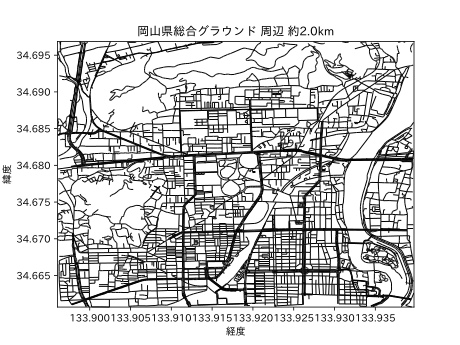
\includegraphics[width=.9\textwidth]{road-oka.pdf}
  \caption{実験で用いる道路ネットワーク}
  \label{fig:road-okayama}
\end{figure}

図\ref{fig:exp-road-oka-correlation}は,辺をひとつ追加したときの,
媒介中心性の最大値の分布である.
辺の追加によって,最大$0.1607$の正規化された媒介中心性を
$0.1379$まで減少させることに成功した.

具体的に,どこに挿入すれば媒介中心性が下がるのかは
図\ref{fig:road-okayama-minmax}に示している.

\begin{figure}[tb]
  \centering
  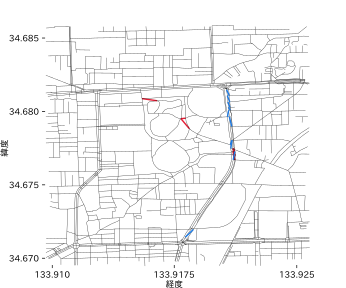
\includegraphics[width=\textwidth]{road-oka-minmax.pdf}
  \caption{青は媒介中心性の最大値が下がり,赤は媒介中心性の最大値が上がる,
  それぞれベスト10を示している}
  \label{fig:road-okayama-minmax}
\end{figure}

\begin{figure}[tb]
  \centering
  \includegraphics[width=.7\textwidth]{exp-road-oka-correlation.pdf}
  \caption{媒介中心性の最大値の分布}
  \label{fig:exp-road-oka-correlation}
\end{figure}

\begin{figure}[tb]
  \centering
  \includegraphics[width=.7\textwidth]{exp-road-oka-time.pdf}
  \caption{計算時間の積算の比較}
  \label{fig:exp-road-oka-time}
\end{figure}

\subsection{媒介中心性のリアルタイム監視}
\label{subsect:exp-sfhh}

第\ref{chap:introduction}章で説明したように,ソーシャルネットワーク分析に
おいて,媒介中心性をはじめとした中心性に注目することが重要である.
しかしながら,現実のソーシャルネットワーキングサイトでは,友人関係が
刻一刻と現れ消えている.この実験では,友人関係の生成/消滅が頻繁に起こりうる
状況で,媒介中心性をリアルタイムで監視する用途への応用を想定する.

この実験では,SFHH\cite{Genois2018}というデータセットを用いた.
このデータセットは,ある会議の開催期間中に,参加者に赤外線タグを持たせ,
参加者同士の交流のパターンを記録したものである.

図\ref{fig:exp-sfhh}は,そのSFHHデータセットをもとに,辺の挿入と削除を
繰り返したときの,各手法の実行時間を表す.それとともに,実時間($20$秒間)の
うちに発生した,挿入と削除操作の内訳を示す.
図より,更新の量が多い場合,提案手法の方が時間がかかることが分かる.
今後は,多くの辺の操作に対応するアルゴリズムの開発が求められる.

\begin{figure}[tb]
  \centering
  \includegraphics[width=.9\textwidth]{exp-sfhh.pdf}
  \caption{SFHHに対する実験結果}
  \label{fig:exp-sfhh}
\end{figure}
